\chapter{Solución}
\label{Solución}

Este capítulo describe el sistema construido: qué se ha desarrollado, con qué arquitectura, cómo se
ha implementado y qué pruebas garantizan que cada eslabón hace lo que dice hacer. Es el capítulo más
extenso de la memoria porque el trabajo no consiste en aplicar un modelo a un conjunto de datos ya
existente, sino en construir la tarea, el conjunto de datos y el banco de evaluación desde cero.


\section{Descripción de la solución}

Visión de conjunto antes del detalle. Lo desarrollado es un \textbf{banco de comparación de
políticas de manipulación}: un entorno de simulación con una tarea instrumentada, una cadena de
captura y conversión de demostraciones, dos vías de entrenamiento que consumen el mismo conjunto de
datos, y un protocolo de evaluación que sirve a ambas a través de la misma interfaz.

\begin{figure}[htb]
\centering
  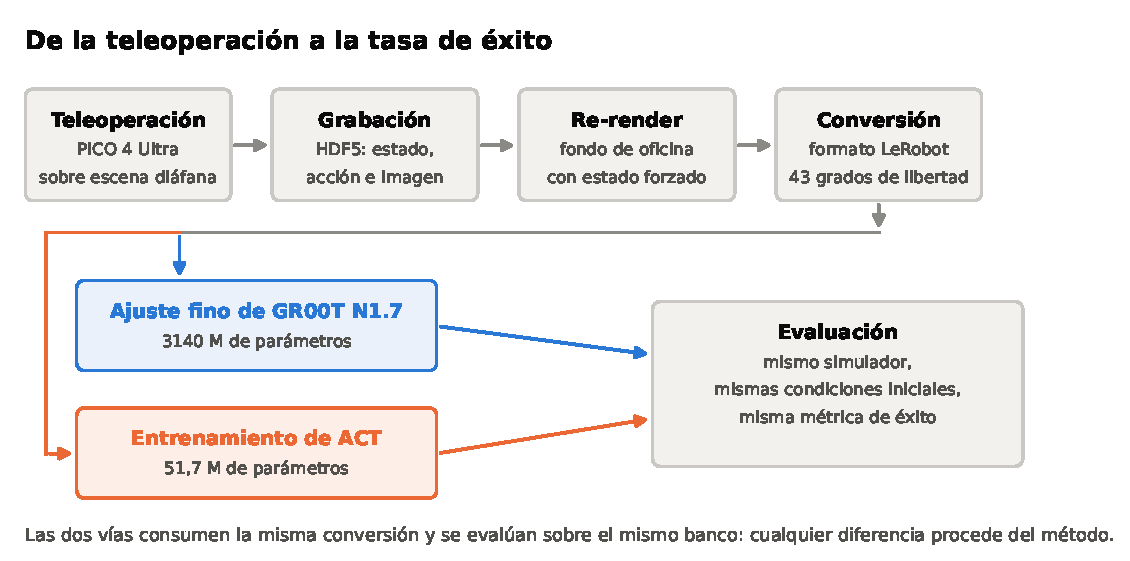
\includegraphics[width=\textwidth]{figuras/sistema/pipeline.pdf}
  \caption[Cadena completa del sistema]{Cadena completa: teleoperación, grabación, conversión,
  entrenamiento por las dos vías y evaluación sobre el mismo simulador}
  \label{fig:pipeline}
\end{figure}


\section{El proceso de desarrollo}

El desarrollo ha seguido un modelo iterativo e incremental, con ciclos cortos cerrados por una
verificación ejecutable. La justificación es específica del dominio: en una cadena de cinco etapas
donde cada una consume la salida de la anterior, un error silencioso en un eslabón temprano invalida
todo el trabajo posterior sin producir ningún síntoma visible. El desarrollo se ordena, por tanto,
de modo que cada etapa quede verificada antes de invertir esfuerzo en la siguiente.

\subsection{Análisis}

\subsubsection{Definición de requisitos}

Enumeración de los requisitos del sistema, divididos en funcionales y no funcionales.

\begin{table*}[ht]
	\centering
	\caption{Requisitos funcionales}
	\label{tab:requisitos-funcionales}
	\makebox[\textwidth]{
		\begin{tabular}{|l|p{11cm}|}
			\cline{1-2}
			Código & Descripción \\ \hline
			RF-01 & [PENDIENTE: la tarea debe poder teleoperarse y grabarse] \\
			RF-02 & [PENDIENTE: criterio de éxito objetivo y automático] \\
			RF-03 & [PENDIENTE: una sola conversión alimenta a los dos métodos] \\
			RF-04 & [PENDIENTE: banco de evaluación común e intercambiable] \\ \hline
		\end{tabular}
	}
\end{table*}

\begin{table*}[ht]
	\centering
	\caption{Requisitos no funcionales}
	\label{tab:requisitos-no-funcionales}
	\makebox[\textwidth]{
		\begin{tabular}{|l|p{11cm}|}
			\cline{1-2}
			Código & Descripción \\ \hline
			RNF-01 & [PENDIENTE: reproducibilidad] \\
			RNF-02 & [PENDIENTE: latencia compatible con el lazo de control] \\
			RNF-03 & [PENDIENTE: trazabilidad de datos y modelos] \\ \hline
		\end{tabular}
	}
\end{table*}

\subsubsection{Especificación de requisitos}

Análisis de los requisitos desde el punto de vista del comportamiento, la estructura y la
funcionalidad del sistema, con los casos de uso principales: capturar una sesión de demostraciones,
convertir un conjunto de datos, entrenar una política y evaluarla.

\subsection{Diseño}

\subsubsection{Diseño de sistema}

Arquitectura y tecnologías. El sistema se reparte entre un contenedor que aloja el simulador y dos
entornos de ejecución independientes para cada método de aprendizaje, comunicados con el simulador
mediante un protocolo de mensajería. Esa separación no es estética: las bibliotecas de aprendizaje
fijan versiones de sus dependencias que son incompatibles con las que exige el simulador, de modo
que instalarlas juntas rompería la herramienta necesaria para evaluar.

\begin{figure}[htb]
\centering
  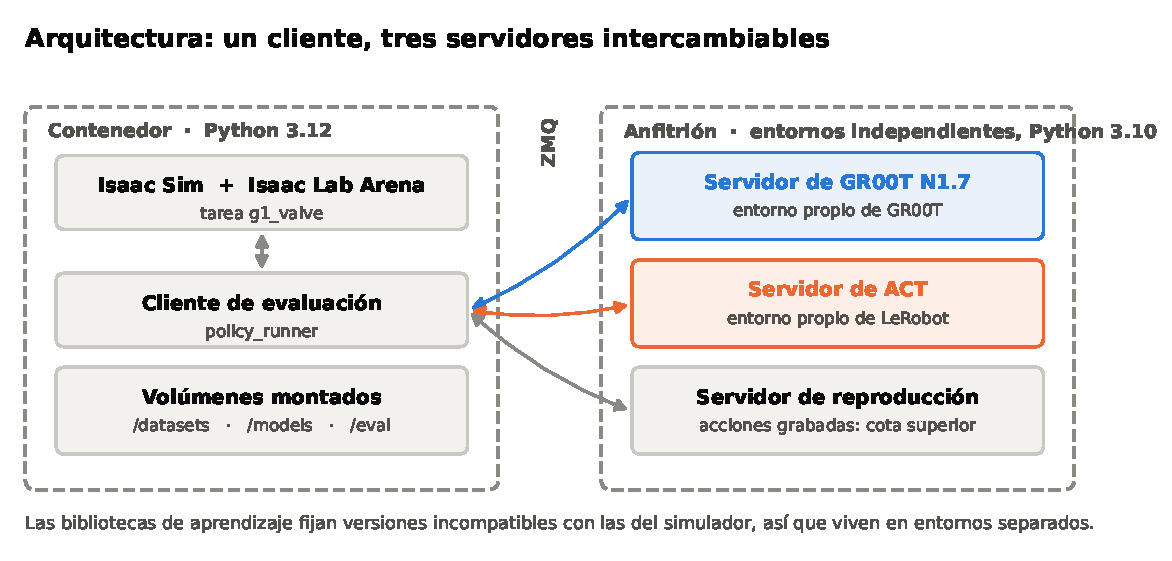
\includegraphics[width=\textwidth]{figuras/sistema/arquitectura.pdf}
  \caption[Arquitectura del sistema]{Arquitectura del sistema: contenedor de simulación, entornos de
  ejecución de cada política y comunicación entre ambos}
  \label{fig:arquitectura}
\end{figure}

\begin{table*}[ht]
	\centering
	\caption{Tecnologías empleadas y versiones}
	\label{tab:tecnologias}
	\makebox[\textwidth]{
		\begin{tabular}{|l|l|p{7cm}|}
			\cline{1-3}
			Componente & Versión & Función \\ \hline
			[PENDIENTE] & & \\ \hline
		\end{tabular}
	}
\end{table*}

\subsubsection{Diseño detallado}

Diseño de la tarea de simulación, de la representación de los datos y de la interfaz de las
políticas.

\paragraph{La tarea de simulación.} Escena, robot, válvula y criterio de éxito. Se detalla aquí la
elección de las dos disposiciones de la válvula, la aleatorización de su posición y el
procedimiento de medida con el que se han fijado todas las poses del entorno.

\begin{figure}[htb]
\centering
  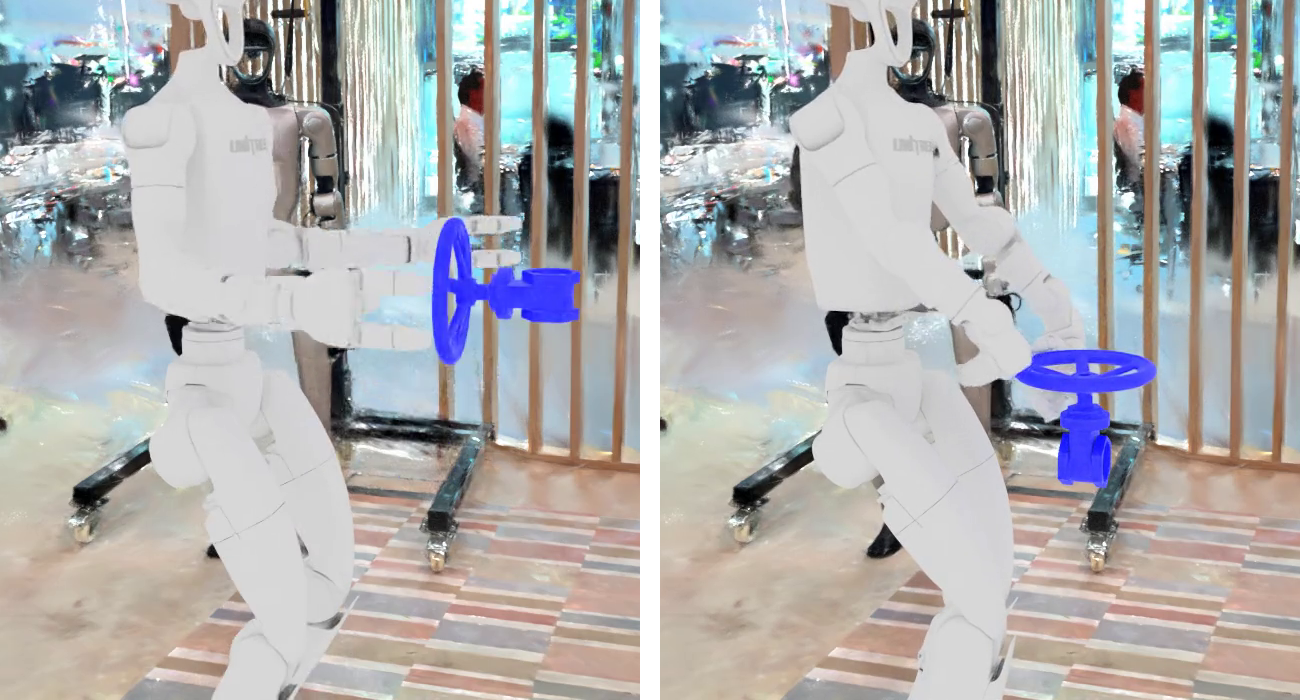
\includegraphics[width=\textwidth]{figuras/simulacion/disposiciones.png}
  \caption[Las dos disposiciones de la válvula]{Las dos disposiciones de la válvula: frontal, con el
  eje de giro horizontal, y cenital, con el eje vertical}
  \label{fig:disposiciones}
\end{figure}

\paragraph{El espacio de acción.} Composición de las veintitrés dimensiones que gobiernan al robot y
discusión de las que resultan degeneradas en el conjunto de datos.

\begin{figure}[htb]
\centering
  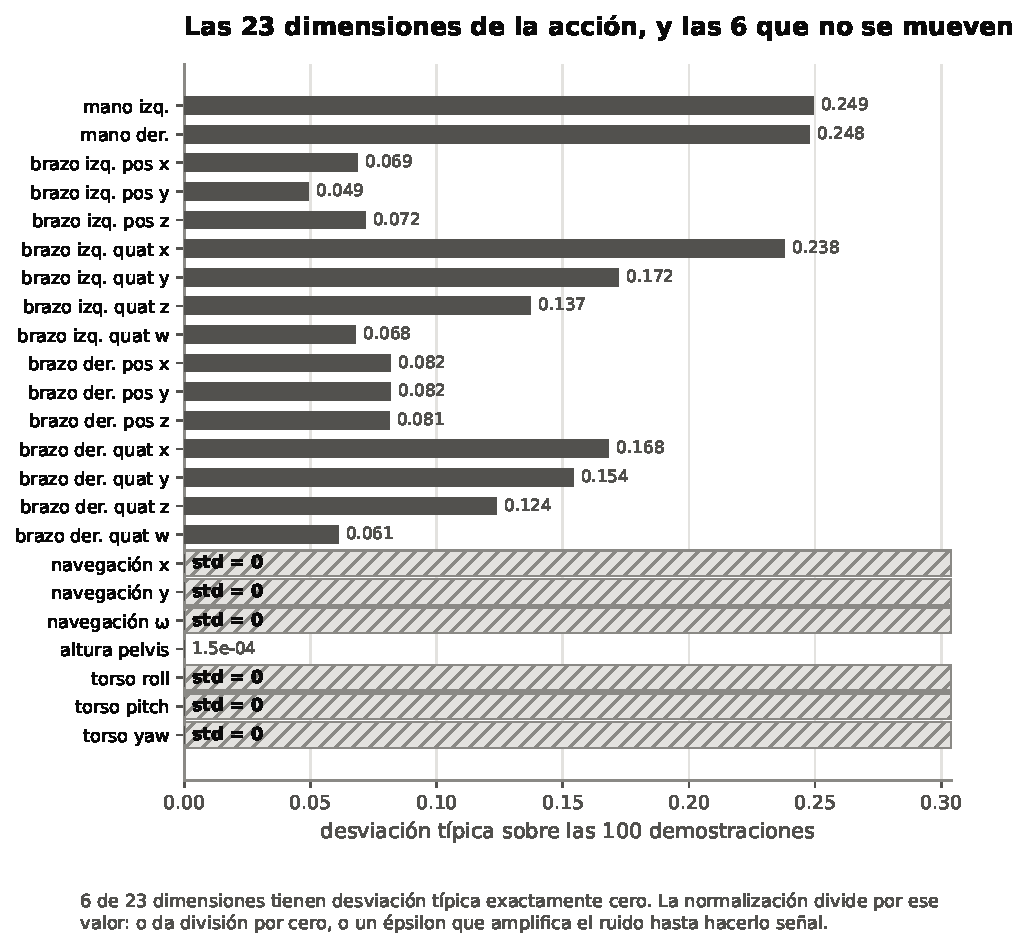
\includegraphics[width=\textwidth]{figuras/resultados/fig7_std_espacio_accion.pdf}
  \caption[Variabilidad de las dimensiones del espacio de acción]{Desviación típica de cada una de
  las veintitrés dimensiones del espacio de acción sobre el conjunto de datos definitivo}
  \label{fig:std-accion}
\end{figure}

\paragraph{El conjunto de datos.} Estructura del formato de almacenamiento y correspondencia entre
la acción de veintitrés dimensiones del simulador y el espacio articular de cuarenta y tres grados
de libertad que consumen las políticas. Se caracteriza aquí el conjunto capturado: cuántas
demostraciones tiene cada sesión, cómo se repartieron entre las dos disposiciones y cuánto dura
cada episodio.

\begin{figure}[htb]
\centering
  
\includegraphics[width=\textwidth]{figuras/resultados/fig5_reparto_disposiciones.pdf}
  \caption[Reparto de disposiciones por sesión]{Reparto de las dos disposiciones de la válvula en
  cada sesión de captura y en el conjunto acumulado}
  \label{fig:reparto-disposiciones}
\end{figure}

\begin{figure}[htb]
\centering
  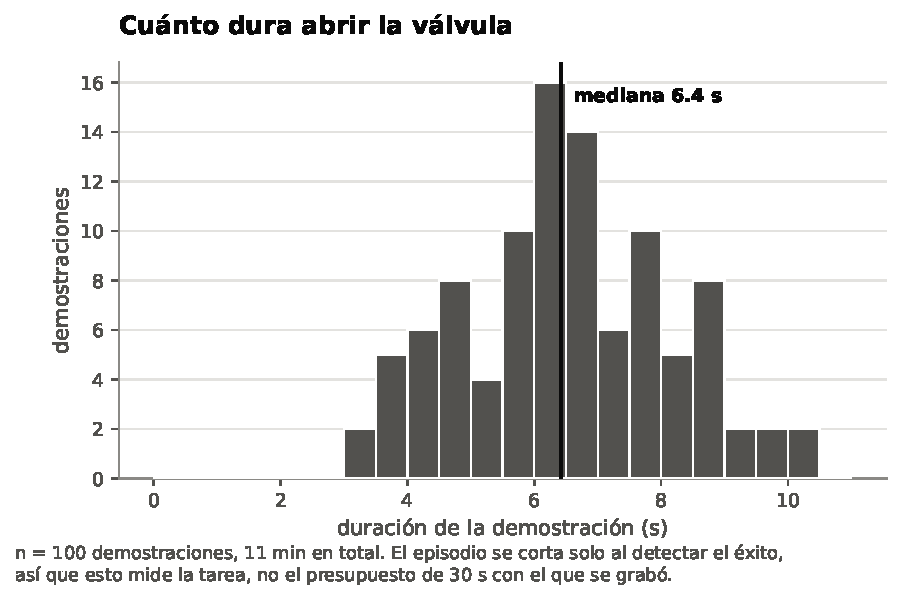
\includegraphics[width=\textwidth]{figuras/resultados/fig6_duracion_episodios.pdf}
  \caption[Duración de las demostraciones]{Distribución de la duración de las demostraciones
  capturadas}
  \label{fig:duracion-episodios}
\end{figure}

\subsection{Implementación}

Herramientas empleadas, organización del proyecto y peculiaridades de la implementación. Esta
sección recoge las decisiones técnicas que condicionaron el resultado y los problemas que hubo que
resolver para que la cadena funcionase: el reescalado de los límites de la articulación de la
válvula, la altura de aparición del robot, la sincronización del sensor de imagen con la
construcción del entorno, la elección del dispositivo de física durante la captura y el
procedimiento de reaplicación del fondo fotorrealista sobre demostraciones ya grabadas.

\begin{figure}[htb]
\centering
  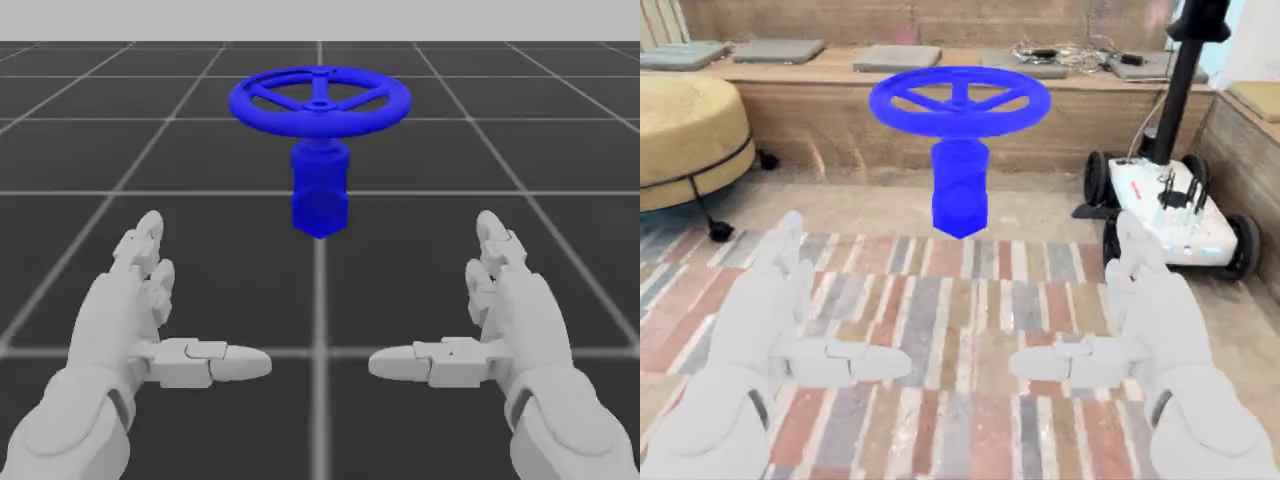
\includegraphics[width=\textwidth]{figuras/simulacion/escenas.png}
  \caption[Escena de captura y escena del conjunto de datos]{Escena diáfana empleada durante la
  teleoperación, frente a la misma demostración con el fondo de oficina reconstruido, que es la que
  llega al conjunto de datos}
  \label{fig:escenas}
\end{figure}

\subsection{Pruebas}

Pruebas realizadas sobre cada eslabón de la cadena, con el resultado de cada una. La pieza central
es la reproducción de las acciones grabadas como cota superior del sistema: si reproducir las
órdenes de una demostración no abre la válvula, ninguna política entrenada sobre ellas lo hará, y
eso debe saberse antes de invertir en la captura masiva.

\begin{table*}[ht]
	\centering
	\caption{Pruebas de verificación de la cadena}
	\label{tab:pruebas}
	\makebox[\textwidth]{
		\begin{tabular}{|l|p{8cm}|l|}
			\cline{1-3}
			Prueba & Qué verifica & Resultado \\ \hline
			[PENDIENTE] & & \\ \hline
		\end{tabular}
	}
\end{table*}


\section{El producto del desarrollo}

Descripción del entregable: el repositorio, su organización, la documentación de lanzamiento y de
entrenamiento, y la forma de ejecutar cada etapa. Se incluyen ejemplos de la interfaz de captura tal
como la ve el operador y de la vista que recibe la política.

\begin{figure}[htb]
\centering
  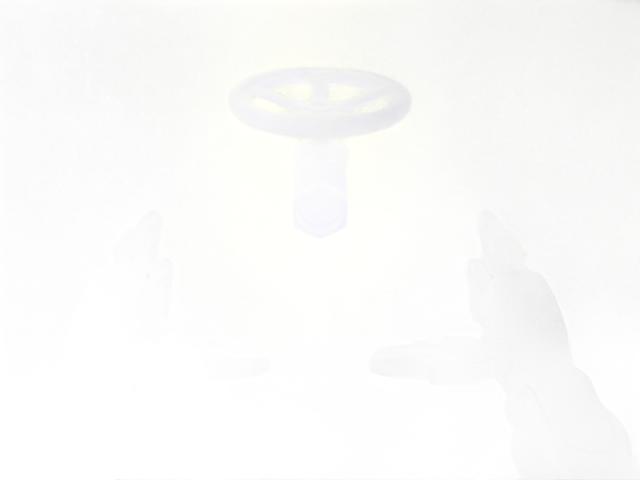
\includegraphics[width=.7\textwidth]{figuras/simulacion/camara_robot.png}
  \caption[Vista de la cámara del robot]{Vista de la cámara de cabeza del robot, que es la única
  entrada visual que recibe la política}
  \label{fig:camara-robot}
\end{figure}
